\section{Introdução}

% ===========================
\begin{frame}{Motivação}
%
\begin{columns}
%
\column{0.35\textwidth}
\begin{figure}
    \centering
    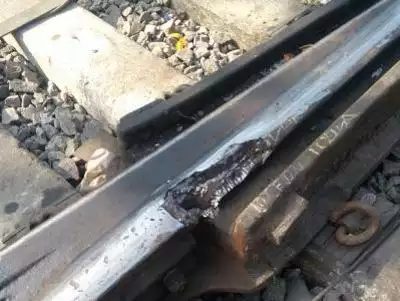
\includegraphics[width=\columnwidth]{figures/dano_trilho.png}
    
    {\footnotesize Fonte: Google Imagens}
\end{figure}
%
\column{0.65\textwidth}
\begin{itemize}
    \item Detecção de danos em trilhos.
    \item Monitoramento da Integridade Estrutural (SHM)
    \item Manutenção preditiva
\end{itemize}
\end{columns}
\begin{block}{Objetivo}
    Desenvolver uma inteligência artificial para fazer a detecção dos danos nos trilhos.
\end{block}
\end{frame}

% ===========================
\begin{frame}{Inteligência Artificial}
\begin{columns}[t]
%
\column{0.3\textwidth}
\begin{block}{Inteligência Artificial}
    Desenvolvimento de sistemas para reconhecimento de fala, visão computacional, planejamento, tomada de decisões e aprendizado.
\end{block}
%
\column{0.3\textwidth}
\begin{block}{Machine Learning}
    Sistema que aprende e melhora automaticamente com base em dados, sem a necessidade de programação explícita. 
\end{block}
%
\column{0.3\textwidth}
\begin{block}{Deep Learning}
    Técnica de machine learning que se concentra em modelos de \alert{redes neurais} profundas para aprender e representar dados.
\end{block}
\end{columns}
\end{frame}
